\chapter{Evaluation and Results}
\label{chapter:evaluation_and_results}



In chapter 4, it was presented the implementation of the proposed solution, giving a description of all the implemented features and how the system should adapt and react in different scenarios, in order to maintain, at least, a minimum functionality, always.

The objective for this chapter is to validate the proposed solution. Firstly, in section \ref{results:scenario}, a deployment scenario overview will be given, highlighting the devices and tools used for that purpose. Following, in section \ref{results:results}, the obtained results for different tests will be analysed. With the requirements, addressed in chapter 3, taken into consideration, the performance of the automation engine, implemented in gateways, will be evaluated, and also, to judge the capacity of the system to react to abnormal functioning scenarios, the reaction time to this occurrences will be measured.

\newpage

\section{Deployment Scenario}
\label{results:scenario}



The final deployment scenario, used to test and validate the system and illustrated in Figure \ref{fig:performance}, is composed by the Building Manager platform, the WSO2 \ac{cep} Engine, the Gateway Manager and two Gateways, all communicating through the MQTT Broker. 

The Building Manager is the component responsible for supporting the user-friendly platform to create rules and distribute devices through the building planer. This platform was hosted in a Linux virtual machine equipped with a single-core processor and 1 gigabyte of memory.

The WSO2 \ac{cep} engine, which is one of the core components of the whole system, as it is the primary processor of events, based on the logic specified in the rules. This component, required a more powerful machine than the Building Manager component , being hosted in a Linux virtual machine with a quad-core processor and 4 gigabytes of memory.

\begin{figure}[H]
	\centering
	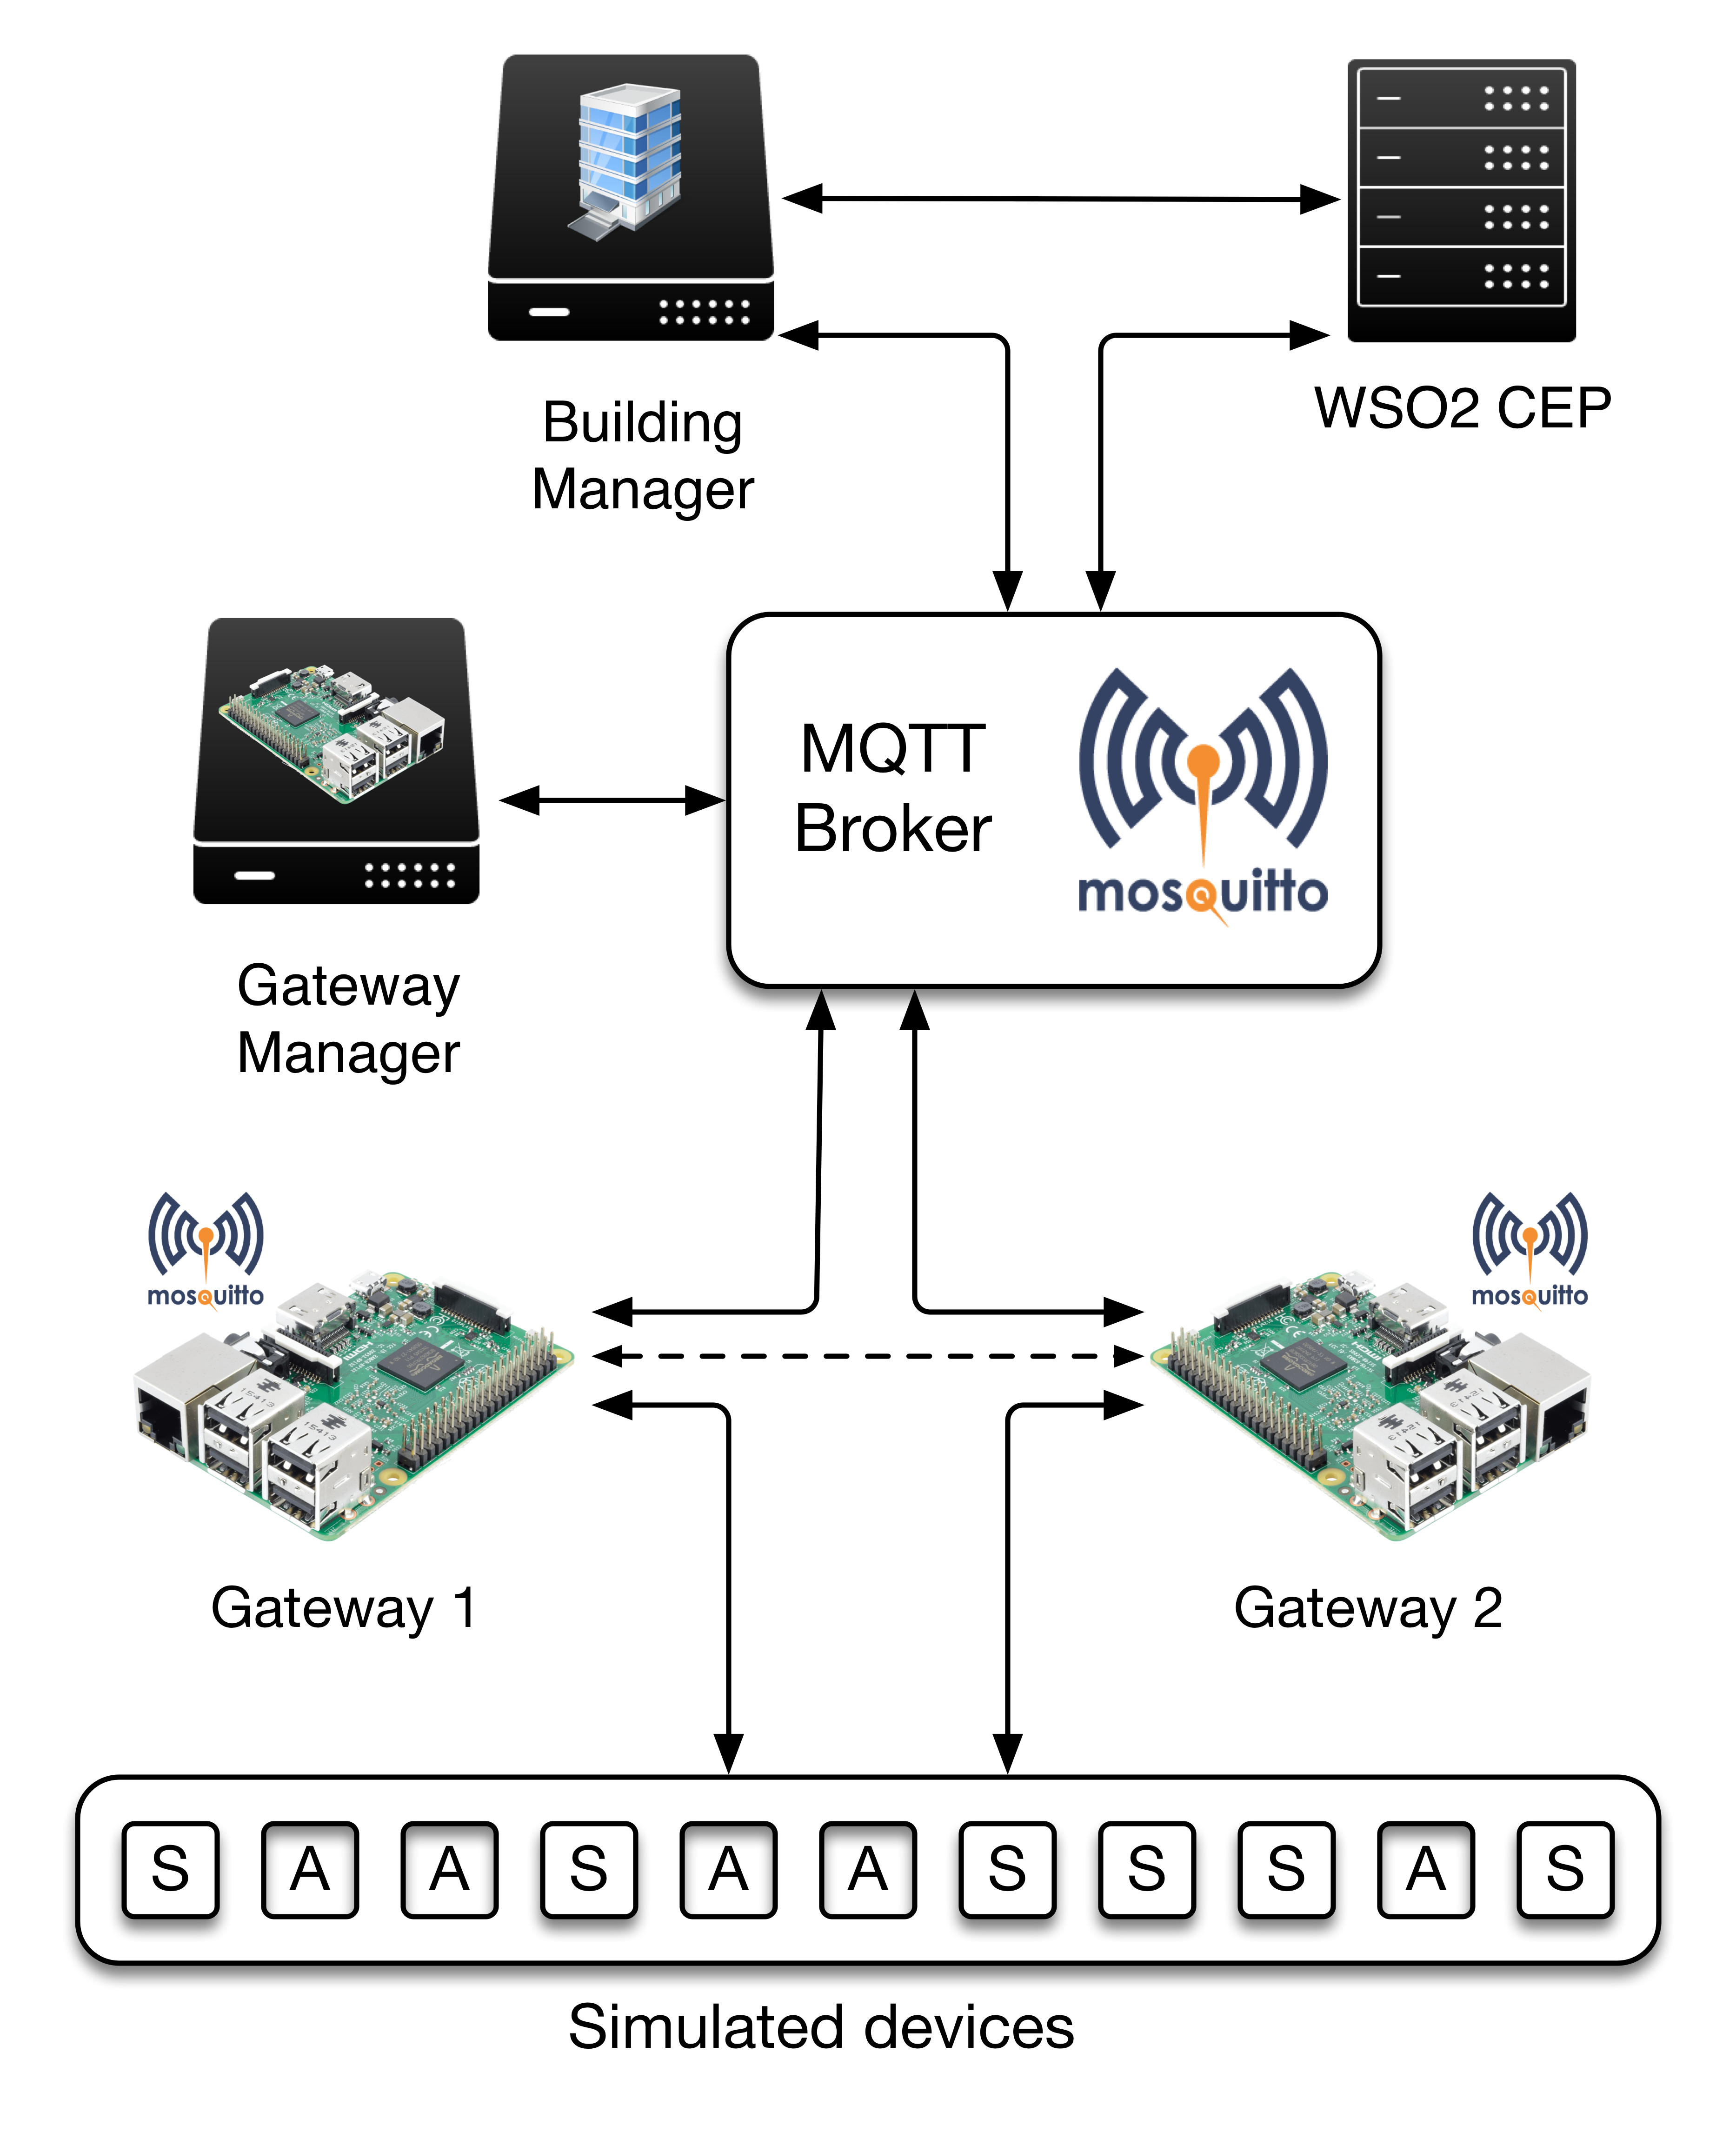
\includegraphics[width=0.7\textwidth]{figures/deployment.png}
	\caption{Deployment Scenario.}
	\label{fig:deploy}
\end{figure}

Regarding the Gateway Manager, it contains both a software for gateway's management and a web-server to offer a platform to check the state of each gateway and the general state of the system. This component was also deployed in a Linux virtual machine with a dual-core processor and 2 gigabytes of memory.

In order to assure the communication between the different components, the Mosquitto MQTT Broker was deployed in a separate virtual machine with a dual-core processor and 2 gigabytes of memory.

Finally, concerning the gateways, which are responsible for communicate with devices and, in some scenarios, process events using its Automation Engine. In this deployment scenario were used simulated devices. To further explain, a equal set of devices were configured in both gateways, simulating a scene where the devices are in range of two different gateways. Each gateway were equipped with code to generate events of the devices assigned to them, by the Gateway Manager. If a gateways had control over a sensor, it should send events with a fixed programmable frequency. This was used for the testing scenario addressed in section \ref{results:fail}%The simulated devices used were motion sensors and lights actuators and it was deployed a rule, to trigger a light on for 5 seconds, each time a motion sensor sends an event. 





\section{Performance Results}
\label{results:results}

In this section will be presented the results and discussion of the tests preformed. Firstly, in section \ref{results:cep} the latency of the gateway's Automation Engine will be mesured and then, in section \ref{results:fail}, the reaction time to system failures will be evaluated.


\subsection{Gateway's Automation Engine Performance}
\label{results:cep}

In order to evaluate the gateway's Automation Engine performance, a stress test was preformed. The objective was to measure the processing time of events, in five different stress situations: first, sending a single event and measure the time taken by the engine to produce an output response, and then increase the number of consecutive events, 10, 100, 1000 and 10000, to not only measure the time taken to process all those events, but also to check if all events were processed. 

For this test, two python scripts were made: one to send a programmable number of events consecutively, and other to measure the time since the first event was sent, and the last response action was received. The deployed rule consisted in inputting a motion event and respond with an event to turn on a light as result. The results of this test are expressed in Figure \ref{fig:performance}.

\begin{figure}[H]
	\centering
	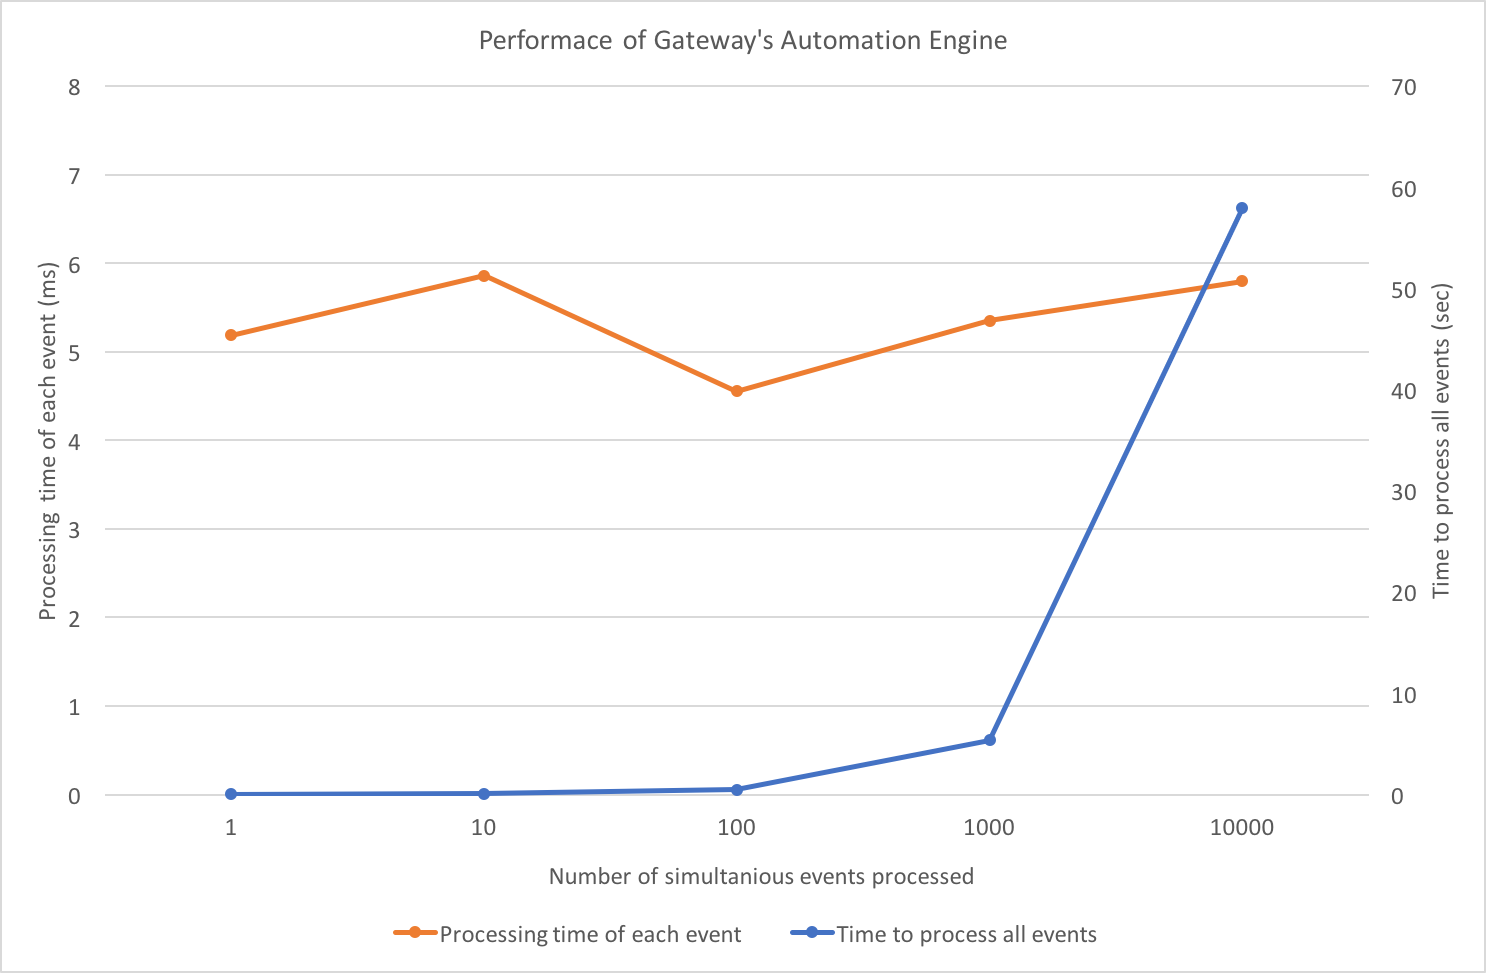
\includegraphics[width=0.9\textwidth]{figures/performance.png}
	\caption{Gateway's Automation Engine Performance.}
	\label{fig:performance}
\end{figure}

\begin{table}[H]
	\centering
	\caption{My caption}
	\label{my-label}
	\begin{tabular}{l|l|l|l|l|l|}
		\cline{2-6}
		& \textbf{1} & \textbf{10} & \textbf{100} & \textbf{1000} & \textbf{10000} \\ \hline
		\multicolumn{1}{|l|}{\textbf{Average Time}}       & 5,2 ms     & 6,9 ms      & 3,7 ms       & 5,3 ms        & 5,8 ms         \\ \hline
		\multicolumn{1}{|l|}{\textbf{Minimum Time}}       & 4,4 ms     & 6,6 ms      & 3,6 ms       & 4,5 ms        & 5,5 ms         \\ \hline
		\multicolumn{1}{|l|}{\textbf{Maximum Time}}       & 6,0 ms     & 7,3 ms      & 3,7 ms       & 6,7 ms        & 6,1 ms         \\ \hline
		\multicolumn{1}{|l|}{\textbf{Standard Deviation}} & 0,7 ms     & 0,3 ms      & 0 ms         & 0,9 ms        & 0,3 ms         \\ \hline
		\multicolumn{1}{|l|}{\textbf{Total Time}}         & 0,005 sec  & 0,069 sec   & 0,367 sec    & 5,350 sec     & 57,953 sec     \\ \hline
	\end{tabular}
	\centering
\caption{Time taken to process each event.}
\label{table:event}
\end{table}

\subsection{System Failure's Reaction Performance}
\label{results:fail}

\begin{table}[H]
	
	\begin{tabular}{|l|l|}
		\hline
		\textbf{Average Time}       & 7,261 sec \\ \hline
		\textbf{Minimum Time}       & 1,185 sec \\ \hline
		\textbf{Maximum Time}       & 5,084 sec \\ \hline
		\textbf{Standard Deviation} & 8,883 sec \\ \hline
	\end{tabular}
	\centering
	\caption{Reaction time to a \ac{cep} Engine failure}
	\label{cepDown}
\end{table}

\begin{table}[H]

	\begin{tabular}{|l|l|}
		\hline
		\textbf{Average Time}       & 13,194 sec \\ \hline
		\textbf{Minimum Time}       & 3,839 sec \\ \hline
		\textbf{Maximum Time}       & 7,492 \\ \hline
		\textbf{Standard Deviation} & 18,877 \\ \hline
	\end{tabular}
	\centering
	\caption{Reaction time to a Gateway failure.}
	\label{gwdown}
\end{table}

\begin{table}[H]
	
	\begin{tabular}{|l|l|}
		\hline
		\textbf{Average Time}       & 0,164 sec \\ \hline
		\textbf{Minimum Time}       & 0,024 sec \\ \hline
		\textbf{Maximum Time}       & 0,129 sec \\ \hline
		\textbf{Standard Deviation} & 0,199 sec \\ \hline
	\end{tabular}
	\centering
	\caption{Reaction time to a Gateway back up.}
	\label{gwup}
\end{table}


Reaction time < 100 ms -> imperceptible 
Miller1968